\documentclass[a4paper, 11pt]{article}
 
\usepackage[utf8]{inputenc}

\usepackage[T1]{fontenc}

\usepackage{graphicx}
\usepackage{float} %H option for figure
\usepackage{hyperref}
\usepackage{listings}
\usepackage{xcolor}


\hypersetup{
    bookmarks=true,
    unicode=true,
    colorlinks=true,        % false: boxed links; true: colored links
    linkcolor=cyan,          % color of internal links (change box color with linkbordercolor)
    citecolor=green,        % color of links to bibliography
    filecolor=magenta,      % color of file links
    urlcolor=cyan           % color of external links
}

\lstset{%configuration de listings
language=TCL, 
float=hbp,% 
basicstyle=\ttfamily\scriptsize, % 
identifierstyle=\color{purple}, % 
keywordstyle=\color{red}, % 
stringstyle=\color{green}, % 
commentstyle=\color{gray}, % 
columns=flexible, % 
tabsize=2, % 
%frame=trBL, % 
%frameround=tttt, % 
extendedchars=true, % 
showspaces=false, % 
showstringspaces=false, % 
numbers=left, % 
numberstyle=\tiny, % 
breaklines=true, % 
breakautoindent=true, % 
captionpos=b,% 
xrightmargin=0cm, % 
xleftmargin=0cm 
}

\parskip 6pt
\parindent 0pt
 
\begin{document}
 
\title{\texttt{smiles\_parser} design document}
\author{Laurent Fasnacht}
%\date{''date de fin de rédaction''} 
 
\maketitle



\newpage
{\parskip 0pt
\tableofcontents

\listoffigures
}
 
\section{Introduction}

\subsection{Intended audience}
The indended audience of this document is both developers interested in using this library, and developers wanting to understand and improve the internals. We assume that the reader is already familiar with SMILES lines.

Section \ref{sec:interface} is probably enough for the first category, while the latter should definitely also read section \ref{sec:internals}.

\subsection{Purpose}

This library, \texttt{smiles\_parser}, is a TCL library to parse \textit{Simplified Molecular Input Line Entry Specification} (SMILES~\cite{SMILES}) into generic and simple to use TCL objects. It was originally written to improve LipidBuilder~\cite{LB}.

Unfortunately there are multiple non-compatible interpretation of what a SMILES is~\cite{OEChem_TK_SMILES_impl}. Therefore, this library was written to support the {OpenSMILES} specification~\cite{OpenSMILES}, which is well-defined and quite common.

\subsection{Example}

Throughout this document, we will use the example of Vanilline, which is represented in figure~\ref{fig:vanillin}. We will also use the following color convention:
\begin{itemize}
    \item Chain numbers: black
    \item Atom numbers: {\color{red}red}
    \item Bond numbers: {\color{blue}blue}
\end{itemize}

\begin{figure}[H]
    \begin{center}
        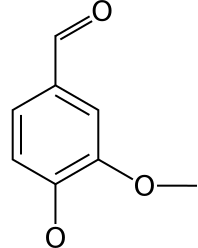
\includegraphics[width=0.4\columnwidth]{images/Vanillin.pdf}
    \end{center}
    \caption[Vanillin molecule]{\label{fig:vanillin} Representation of the vanillin molecule, {\tt O=Cc1ccc(O)c(OC)c1}.}
\end{figure}


\section{Interface}\label{sec:interface}


\subsection{Representations}

There are various way of representing a parsed SMILES string. Two of them were chosen, and will be presented thereafter.

\subsubsection{Tree structure}

The most natural way is a tree structure, because it directly arise from the specification. It is also the easiest structure to create (except finding the neighbors, which is quite difficult), and correspond closely to the string.

It's important to notice that it has the major drawback that it's difficult and computationnaly expensive to locate an element (i.e. ``where's atom 9?''), because the only straightforward way to do this is recursive.

You can see in figure~\ref{fig:vanillin-tree} the tree representation of the vanillin molecule (fig.~\ref{fig:vanillin}).

\begin{figure}
    \begin{center}
        \includegraphics[width=0.8\columnwidth]{images/Vanillin-tree.pdf}
    \end{center}
    \caption[Tree representation of the vanillin molecule]{\label{fig:vanillin-tree} Tree representation of the vanillin molecule, {\tt O=Cc1ccc(O)c(OC)c1}. The atoms are carbon, unless otherwise specified. The gray arrows are "neighbors" indication.}
\end{figure}

\subsubsection{Flat structure}

To be able to quickly use the data, it is required to have a more efficient alternative. Since TCL doesn't have pointers, we need to duplicate data.

Therefore, we can define 3 lists:
\begin{itemize}
    \item List of chains ({\tt chain[0]} is the full tree, like in figure \ref{fig:vanillin-tree})
    \item List of bonds
    \item List of atoms, including their subtree.
\end{itemize}

To have an intuitive view, you can look at figure~\ref{fig:vanillin-flat}.

\begin{figure}
    \begin{center}
        \includegraphics[width=0.8\columnwidth]{images/Vanillin-flat.pdf}
    \end{center}
    \caption[Flat representation of the vanillin molecule]{\label{fig:vanillin-flat} Flat representation of the vanillin molecule, {\tt O=Cc1ccc(O)c(OC)c1}. The clusters represents the different table elements. Clusters for bonds were omitted (as they only return the bond).}
\end{figure}

\subsection{Objects}
Every object is implemented as a list. The first entry of the list is the type:
\begin{itemize}
    \item \texttt{"chain"}
    \item \texttt{"bond"}
    \item \texttt{"ringbond"}
    \item \texttt{"atom"}
\end{itemize}

The next elements depend on the type, and will be defined in the corresponding subsection below. A general remark is that you shouldn't do direct indexing (except for the first entry, the type), and instead use the constants defined at the beginning of \texttt{smiles\_parser.tcl}. By doing this way, you ensure that your code would not break if some field is added to the structure later on. For instance:

\lstinputlisting{codesamples/indexing.tcl}

\subsubsection{Chain}\label{subsubsec:chain}

A chain is an list of bond and atoms. The object has the following attributes:
\begin{itemize}
    \item \texttt{chain\_id}: ID of the chain. Unique. Chain 0 is at the highest level.
    \item \texttt{chain\_atomcount}: Number of atoms in the whole subtree of this chain.
    \item \texttt{chain\_bondcount}: Number of bonds in the whole subtree of this chain.
    \item \texttt{chain\_chaincount}: Number of chain in the whole subtree of this chain (includes this element. E.g. a chain containing no subchain will have a \texttt{chaincount} of 1).
    \item \texttt{chain\_list}: List of elements (atom or bonds) which belong directly to this chain.
\end{itemize}

\subsubsection{Bond}\label{subsubsec:bond}

\begin{itemize}
    \item \texttt{bond\_id}: ID of the bond. Unique.
    \item \texttt{bond\_count}: Multiplicity of the bond. 
    \begin{itemize}
        \item \texttt{-}, \texttt{/}, \texttt{:}, \texttt{\textbackslash}, (implicit), $\Rightarrow 1$
        \item \texttt{=} $\Rightarrow 2$
        \item \texttt{\#} $\Rightarrow 3$
        \item \texttt{\$} $\Rightarrow 4$
    \end{itemize}
    \item \texttt{bond\_aromatic}: Is the bond aromatic?
    \begin{itemize}
        \item yes (explicit \texttt{:}, or implicit between two aromatic atoms) $\Rightarrow 1$
        \item no (explicit \texttt{-}, or implicit not between two aromatic atoms) $\Rightarrow 0$
    \end{itemize}
    \item \texttt{bond\_direction}: Contains information for cis-trans like \texttt{/} or \texttt{\textbackslash} (\texttt{-} if not specified, even for multiple bonds or aromatic)
    \item \texttt{bond\_linking}: List containing the two atom IDs linked by this bond.
\end{itemize}

\subsubsection{Atom}\label{subsubsec:atom}

\begin{itemize}
    \item \texttt{atom\_id}: ID of the atom. Unique.
    \item \texttt{atom\_atomcount}: (total) number of atom in branches (does NOT include the current atom)
    \item \texttt{atom\_bondcount}: (total) number of bond in branches
    \item \texttt{atom\_chaincount}: (total) number of chain in branches
    \item \texttt{atom\_symbol}: Chemical symbol of the atom (always in capital form, even for aromatic), or \texttt{*}
    \item \texttt{atom\_aromatic}: Is the atom aromatic?
    \begin{itemize}
        \item yes $\Rightarrow 1$
        \item no $\Rightarrow 0$
    \end{itemize}
    \item \texttt{atom\_isotope}: Isotope of the atom. -1 if not specified.
    \item \texttt{atom\_chiral}: Chiral part of the atom specification
    \item \texttt{atom\_hcount}: Number of hydrogen
    \item \texttt{atom\_charge}: Charge, as an integer
    \item \texttt{atom\_class}: Atom class (integer)
    \item \texttt{atom\_ringbonds}: List of ringbonds connected to this atom (only exist for the second part of the link, to avoid duplicate)
    \item \texttt{atom\_branches}: List of chains, which are branches starting from this atom.
    \item \texttt{atom\_linkedby}: List of bond IDs connected to this atom.
\end{itemize}

\subsubsection{Ringbonds}

\begin{itemize}
    \item \texttt{ringbond\_number}: Number used to declare the ringbond
    \item \texttt{ringbond\_ref}: Reference counter (the same ringbond number can be used multiple time according to the specification. This number will increase each time it is reused)
    \item \texttt{ringbond\_bond}: The corresponding bond (as defined in \ref{subsubsec:bond})
    \item \texttt{ringbond\_toatom}: (\textbf{\color{red} PRIVATE, DO NOT USE!}) Only for internal usage, use bond attribute instead (contains the target atom ID).
\end{itemize}

\subsection{Functions}

This library only export two public function. You should not try to call another function, as they are reserved for internal use.

\subsubsection{\tt ::smiles\_parser::smiles\_parse}\label{subsubsec:intf_smiles_parse}

This function takes one argument, the SMILES string (which should be valid according to the OpenSMILES specification~\cite{OpenSMILES}), and returns the corresponding tree structure.

It may abort ({\tt error}) if something is wrong, like:
\begin{itemize}
    \item The SMILES string is invalid (two bonds one after the other, invalid atom, etc.)
    \item An explicit aromatic bond was written between two non-aromatic atoms.
    %TODO Add other exceptions
\end{itemize}

\subsubsection{\tt ::smiles\_parser::flatten}\label{subsubsec:intf_flatten}

This function takes as argument the tree returned by {\tt ::smiles\_parser::smiles\_parse}, and returns the corresponding flat structure.

When used correctly, it should never fail.

\subsection{Example}

Here's an example of running with the vanillin molecule:

\lstinputlisting{../test/test_vanillin.tcl}

You can run this file by going in the \texttt{test} folder, and launching: \\
\texttt{tclsh test\_vanillin.tcl}

\section{Internals}
\label{sec:internals}
\subsection{Callgraph}

\begin{figure}[H]
    \begin{center}
        \includegraphics[width=\columnwidth]{images/callgraph.pdf}
    \end{center}
    \caption[Callgraph]{\label{fig:callgraph} Callgraph the defined functions. Functions with gray background are the ones belonging to the interface. Functions starting with an underscore are private functions. \texttt{smiles\_parse\_chain}, \texttt{smiles\_parse\_atom} and \texttt{smiles\_parse\_bond} are not public, in the sense that they are not really useful by themselves, but may still be used without any side effects.}
\end{figure}


\subsection{Description of the functions}

In this section, we will briefly describe the intent which of the functions.

\subsubsection{\tt smiles\_parse}\label{internal:smiles_parse}
The interface was already described in part~\ref{subsubsec:intf_smiles_parse}. This basically do the following:
\begin{enumerate}
    \item Parses the SMILES ({\tt smiles\_parse\_chain}~\ref{internal:smiles_parse_chain})
    \item Number the different elements ({\tt \_chain\_renumber}~\ref{internal:_chain_renumber})
    \item Flatten the structure ({\tt flatten}~\ref{internal:flatten})
    \item Find neighbors ({\tt \_chain\_find\_neighbors}~\ref{internal:_chain_find_neighbors}). It's easier to do so on if we can index directly.
    \item Update the tree using information from the flattened structure. ({\tt \_unflatten}~\ref{internal:_unflatten})
\end{enumerate}

\subsubsection{\tt flatten}\label{internal:flatten}

The interface was already described in part~\ref{subsubsec:intf_flatten}.

It is really simple: it initialize the internal variables for {\tt \_flatten}~(\ref{internal:_flatten}), calls it, and returns the result.

\subsubsection{\tt smiles\_parse\_chain}\label{internal:smiles_parse_chain}

This function accepts a SMILES string and a boolean as parameters. The boolean indicates if the string should start with a bond (like in a branch) or not (main SMILES string).

The function returns a list containing the length parsed, and a \texttt{chain} (\ref{subsubsec:chain}) object.

{\tt smiles\_parse\_chain} tries to alternatively parse an atom ({\tt smiles\_parse\_atom}~\ref{internal:smiles_parse_atom}) and a bond ({\tt smiles\_parse\_bond}~\ref{internal:smiles_parse_bond}). If for some reason one of these function fails, it either throws an error, or stops and returns what was parsed till now.

\subsubsection{\tt smiles\_parse\_atom}\label{internal:smiles_parse_atom}

This function accepts a SMILES string as an argument, which is expected to start by an atom. It returns the length parsed and an \texttt{atom} (\ref{subsubsec:atom}) object.

Basically, it first tries to parse the real "atom" part, and then tries to find ringbonds (using {\tt smiles\_parse\_bond}~\ref{internal:smiles_parse_bond} to parse them), and finally parses the branches (using {\tt smiles\_parse\_chain}~\ref{internal:smiles_parse_chain} with the chain between the parentheses, and 1 as the second argument, since the branch should start by a bond).

\subsubsection{\tt smiles\_parse\_bond}\label{internal:smiles_parse_bond}

This function accepts a SMILES string as an argument, which is expected to start by an bond (which may be implicit). It returns the length parsed and an \texttt{bond} (\ref{subsubsec:bond}) object. Note that the length parsed may be 0 (if the bond is implicit).

\subsubsection{\tt \_chain\_renumber}\label{internal:_chain_renumber}

This function numbers the object provided using a recursive DFS strategy. It also resolves the ringbonds (only the second reference to a number remains, which mean that "open" ringbonds are discarded.

It returns the numbered object.

It uses the following global variables:
\begin{itemize}
    \item \texttt{::smiles\_parser::cur\_id\_atom}
    \item \texttt{::smiles\_parser::cur\_id\_bond}
    \item \texttt{::smiles\_parser::cur\_id\_chain}
    \item \texttt{::smiles\_parser::cur\_ringbond\_links}.
\end{itemize}

While these three first variables only hold the id for the next element, the latter is a cache (dictionnary) to resolve the ringbonds. All these variables should be initialized before calling this function. See the source code of \texttt{smiles\_parse} to see how.

\subsubsection{\tt \_chain\_find\_neighbors}\label{internal:_chain_find_neighbors}

This function accepts a chain, and (facultative, if this is a branch) the previous atom ID. It traveses everything (DFS strategy), calling \\{\tt \_chain\_find\_neighbors\_add\_link}~(\ref{internal:_chain_find_neighbors_add_link}) for any link it discovers.

\subsubsection{\tt \_chain\_find\_neighbors\_add\_link}\label{internal:_chain_find_neighbors_add_link}

This function has three arguments:
\begin{enumerate}
    \item The first atom ID
    \item The bond ID
    \item The second atom ID
\end{enumerate}

It updates in the cache (\texttt{::smiles\_parser::cur\_flatten\_*}, see~\ref{internal:_flatten}):
\begin{itemize}
    \item For the bond: \tt{bond\_linking} attribute
    \item For atoms: \tt{atom\_linkedby} attribute
\end{itemize}

It also updates the bond to set it aromatic if both atoms are aromatic and the bond was implicit, and checks if the bond was specified aromatic that both ends are indeed aromatic.

Note that you'll have to call {\tt \_unflatten} (\ref{internal:_unflatten}) afterwards to recreate the full tree, with the new information.

\subsubsection{\tt \_flatten}\label{internal:_flatten}

This function takes object provided as an argument, and by doing recursively a DFS, update the cache for the flattened structure. It also returns the new state of the cache. (list containing three elements: the list of atoms, the list of bonds, and the list of chains)

The cache is composed of three global variables:
\begin{itemize}
    \item \texttt{::smiles\_parser::cur\_flatten\_atom}
    \item \texttt{::smiles\_parser::cur\_flatten\_bond}
    \item \texttt{::smiles\_parser::cur\_flatten\_chain}
\end{itemize}

Basically, the idea is to set \texttt{::smiles\_parser::cur\_flatten\_atom[x]} to be the atom with id \texttt{x}.

The cache should be initialized to a list of the correct size before calling this function. See for instance the source code of {\tt flatten} (\ref{internal:flatten}).

\subsubsection{\tt \_unflatten}\label{internal:_unflatten}

This function takes as argument an element, and updates every element using the data from the cache (see \ref{internal:_flatten}).

It uses a DFS strategy. It is very important to first replace the element, and then do the recursion, as the cache may be unconsistent (we only update the top level object in the cache, so the subtree of one of its element is may not correspond).


 
\begin{thebibliography}{9}

\bibitem{LB}
    LipidBuilder,\\
    \url{http://lipidbuilder.epfl.ch/}
      
\bibitem{SMILES}
    SMILES,\\
    \url{http://www.epa.gov/med/Prods_Pubs/smiles.htm}
    
\bibitem{OEChem_TK_SMILES_impl}
    SMILES Line Notation, OEChem TK,\\
    \url{http://www.eyesopen.com/docs/toolkits/current/html/OEChem_TK-python/SMILES.html}
    
\bibitem{OpenSMILES}
    OpenSMILES Specification,\\
    \url{http://www.opensmiles.org/opensmiles.html}
    
\end{thebibliography}
\end{document}
